\documentclass[ucs,10pt]{beamer}

\usepackage[utf8]{inputenc}
\usepackage[english]{babel}
\usepackage{graphicx}


% Bla bla bla
% Das Template hab ich ein bisschen anpassen muessen, da pgfdeclareimage usw. irgendwie
% nicht mehr funktionieren wollte. Moeglicherweise aufgrund einer neuen Version o.Ae.
% So gehts aber auch.


% Template for talks using the Corporate Design of the Freie Universitaet
%   Berlin, created following the guidelines on www.fu-berlin.de/cd by
%   Tobias G. Pfeiffer, <tobias.pfeiffer@math.fu-berlin.de>
% This file can be redistributed and/or modified in any way you like.
%   If you feel you have done significant improvements to this template,
%   please consider providing your modified version to
%   https://www.mi.fu-berlin.de/w/Mi/BeamerTemplateCorporateDesign

% NOTE: Removed pgf because it didn't work for me.

%%% FU logo
% small version for upper right corner of normal pages
%\pgfdeclareimage[height=0.9cm]{university-logo}{FULogo_RGB}
%\logo{\pgfuseimage{university-logo}}
% large version for upper right corner of title page
%\pgfdeclareimage[height=1.085cm]{big-university-logo}{FULogo_RGB}
%\newcommand{\titleimage}[1]{\pgfdeclareimage[height=2.92cm]{title-image}{#1}}
%\titlegraphic{\pgfuseimage{title-image}}
%%% end FU logo

\logo{
\includegraphics[height=0.9cm]{FULogo_RGB.png}}
\newcommand{\titleimage}[1]{\titlegraphic{\includegraphics[height=2.92cm]{#1}}}

% NOTE: 1cm = 0.393 in = 28.346 pt;    1 pt = 1/72 in = 0.0352 cm
\setbeamersize{text margin right=2.5mm, text margin left=7.5mm}  % text margin

% colors to be used
\definecolor{text-grey}{rgb}{0.45, 0.45, 0.45} % grey text on white background
\definecolor{bg-grey}{rgb}{0.66, 0.65, 0.60} % grey background (for white text)
\definecolor{fu-blue}{RGB}{0, 51, 102} % blue text
\definecolor{fu-green}{RGB}{153, 204, 0} % green text
\definecolor{fu-red}{RGB}{204, 0, 0} % red text (used by \alert)

% switch off the sidebars
% TODO: loading \useoutertheme{sidebar} (which is maybe wanted) also inserts
%   a sidebar on title page (unwanted), also indents the page title (unwanted?),
%   and duplicates the navigation symbols (unwanted)
\setbeamersize{sidebar width left=0cm, sidebar width right=0mm}
\setbeamertemplate{sidebar right}{}
\setbeamertemplate{sidebar left}{}
%    XOR
% \useoutertheme{sidebar}

% frame title
% is truncated before logo and splits on two lines
% if neccessary (or manually using \\)
\setbeamertemplate{frametitle}{%
    \vskip-30pt \color{text-grey}\large%
    \begin{minipage}[b][23pt]{80.5mm}%
    \flushleft\insertframetitle%
    \end{minipage}%
}

%%% title page
% TODO: get rid of the navigation symbols on the title page.
%   actually, \frame[plain] *should* remove them...
\setbeamertemplate{title page}{
% upper right: FU logo
\vskip2pt\hfill
\includegraphics[height=1.085cm]{FULogo_RGB} \\
\vskip6pt\hskip3pt
% title image of the presentation
\begin{minipage}{11.6cm}
\hspace{-1mm}\inserttitlegraphic
\end{minipage}

% set the title and the author
\vskip14pt
\parbox[top][1.35cm][c]{11cm}{\color{text-grey}\inserttitle \\ \small \insertsubtitle}
\vskip11pt
\parbox[top][1.35cm][c]{11cm}{ \insertinstitute \\[3mm] \insertdate}
}
%%% end title page

%%% colors
\usecolortheme{lily}
\setbeamercolor*{normal text}{fg=black,bg=white}
\setbeamercolor*{alerted text}{fg=fu-red}
\setbeamercolor*{example text}{fg=fu-green}
\setbeamercolor*{structure}{fg=fu-blue}

\setbeamercolor*{block title}{fg=white,bg=black!50}
\setbeamercolor*{block title alerted}{fg=white,bg=black!50}
\setbeamercolor*{block title example}{fg=white,bg=black!50}

\setbeamercolor*{block body}{bg=black!10}
\setbeamercolor*{block body alerted}{bg=black!10}
\setbeamercolor*{block body example}{bg=black!10}

\setbeamercolor{bibliography entry author}{fg=fu-blue}
% TODO: this doesn't work at all:
\setbeamercolor{bibliography entry journal}{fg=text-grey}

\setbeamercolor{item}{fg=fu-blue}
\setbeamercolor{navigation symbols}{fg=text-grey,bg=bg-grey}
%%% end colors

%%% headline
\setbeamertemplate{headline}{
\vskip4pt\hfill\insertlogo\hspace{3.5mm} % logo on the right

\vskip6pt\color{fu-blue}\rule{\textwidth}{0.4pt} % horizontal line
}
%%% end headline

%%% footline
\newcommand{\footlinetext}{\insertshortinstitute, \insertshorttitle, \insertshortdate}
\setbeamertemplate{footline}{
\vskip5pt\color{fu-blue}\rule{\textwidth}{0.4pt}\\ % horizontal line
\vskip2pt
\makebox[123mm]{\hspace{7.5mm}
\color{fu-blue}\footlinetext
\hfill \raisebox{-1pt}{\usebeamertemplate***{navigation symbols}}
\hfill \insertframenumber}
\vskip4pt
}
%%% end footline


\titleimage{polygons}

\title[Random Polygons]{Random Polygons}
\subtitle{2. Zwischenpräsentation}
%TODO: right?
\institute[FU Berlin]{Freie Universität Berlin}
\date[06.12.2011]{6th December 2011}

\begin{document}

\begin{frame}[plain]
  \titlepage
\end{frame}


\begin{frame}{Goals}
	\begin{itemize}
	\item Testing framework for algorithms related to random polygons
	\item Generate random polygons (fair, representative)
	\item Run shortest path algorithm on polygon
	\item Statistical analysis
	\end{itemize}
\end{frame}

\begin{frame}{2. Milestone}
  \begin{itemize}
  \item accomplish 6.12.-12.12.
  \item all polygon generation algorithms
  \item shortest path algorithm
  \item GUI basic version
  \end{itemize}
\end{frame}

\begin{frame}{Geometry Framework}
  \begin{itemize}
    \item needed for some polygon generation algorithms
    \item existing:
    \begin{itemize}
      \item needed accuracy not given
      \item too big 
      \item partly inconsistent
      \item 
    \end{itemize}
    \item therefore small own implementation
  \end{itemize}
\end{frame}

\begin{frame}{Generation algorithms}
  Permute and Reject \begin{footnotesize}by Auer and Held\end{footnotesize}
  \vspace*{1em}
  \begin{itemize}\begin{small}
    \item[ ] input: size n or n points
    \item[i.] generate points, if necessary
    \item[ii.] permute points
    \item[iii.] test if polygon simple. if not, continue with ii.
  \end{small}\end{itemize}
  \vspace*{1em}
  \begin{itemize}\begin{small}
    \item simple to implement
    \item generates all simple polygons with uniform distribution
    \item runntime depends on polygons needed to be generated to encounter
          simple polygon (max. n=15 for fast results)
    \item not suited for practical use
  \end{small}\end{itemize}
\end{frame}

\begin{frame}{Generation algorithms}
  2opt.-Moves \begin{footnotesize}by Auer and Held\end{footnotesize}
  \vspace*{1em}
  \begin{itemize}\begin{small}
    \item[ ] input: size n or n points
    \item[i.] generate random permutation of n points
    \item[ii.] for every self intersection of two edges $ \overline{ab} $ and $ \overline{cd} $
      \begin{itemize}
        \item[a.] remove $ \overline{ab} $ and $ \overline{cd} $
        \item[b.] insert $ \overline{ac} $ and $ \overline{bd} $
      \end{itemize}
  \end{small}\end{itemize}
  \vspace*{1em}
  \begin{itemize}\begin{small}
    \item needs special treatment for polygons not in general position
    \item generates all polygons, but not with uniform distribution
  \end{small}\end{itemize}
\end{frame}

\begin{frame}{Generation algorithms}
  Space Partitioning \begin{footnotesize}by Auer and Held\end{footnotesize}
  \vspace*{1em}
  \begin{itemize}\begin{small}
    \item[ ] input: set S of n points
    \item[i.] choose points $ s_f, s_t \in S $ at random
    \item[ii.] draw line $ \overline{s_fs_t} $ $ \rightarrow $ 2 sets
    \item[iii.] recursively for all subsets S', $ s_f' $ first, $ s_t' $ last point:
      \begin{itemize}
        \item[a.] if S' only consists of $ s_f' $, $ s_t' $, return $ \overline{s_f's_t'} $
        \item[b.] choose s' from S' at random
        \item[c.] draw random line through s' intersecting $ \overline{s_f's_t'} $, thereby creating subsets S'', S''', first and last point $ s_f', s' $ and $ s', s_t' $
      \end{itemize}
  \end{small}\end{itemize}
  \vspace*{1em}
  \begin{itemize}\begin{small}
    \item generates not every possible simple polygon
    %TODO: why?
  \end{small}\end{itemize}
\end{frame}

\begin{frame}{Generation algorithms}
  Incremental Construction \& Backtracking \begin{footnotesize}by Auer and Held\end{footnotesize}
  \vspace*{1em}
  \begin{itemize}\begin{small}
    \item[ ] input: n points
    \item[i.] set of all possible edges, all unmarked, randomly choose current point s
    \item[ii.] recursively for current point:
    \begin{itemize}
      \item[a.] add next possible unmarked edge to polygon, mark all intersecting edges
      \item[b.] backtrack if no unmarked edges left and incompleted polygon
    \end{itemize}
  \end{small}\end{itemize}
  \vspace*{1em}
  \begin{itemize}\begin{small}
    \item speed depends on backtracking
    \item complex to optimize backtracking
    \item currently not suited for practical use
  \end{small}\end{itemize}
\end{frame}

\begin{frame}{Generation algorithms}
  Generating random Polygons \begin{footnotesize}by O'Rourke and Virmani\end{footnotesize}
  \vspace*{1em}
  \begin{itemize}\begin{small}
    \item[ ] input: size n, radius circle, max. speed, steps t
    \item[i.] generate random points on circle $ \rightarrow $ regular polygon
    \item[ii.] t times:
    \begin{itemize}
      \item[a.] move each vertex with random speed and direction
      \item[b.] test if move violates 2 conditions:
        \begin{itemize}
          \item polygon is simple
          \item vertices in bounding region
        \end{itemize}
      \item[c.] discard last step if violation of conditions
    \end{itemize}
  \end{small}\end{itemize}
  \vspace*{1em}
  \begin{itemize}\begin{small}
    \item still not accessible from GUI
    \item seems to generate specific class of polygons
    \item interesting for statistical analysis
  \end{small}\end{itemize}
\end{frame}

\begin{frame}{Generation algorithms (cont.)}
  \begin{center}
    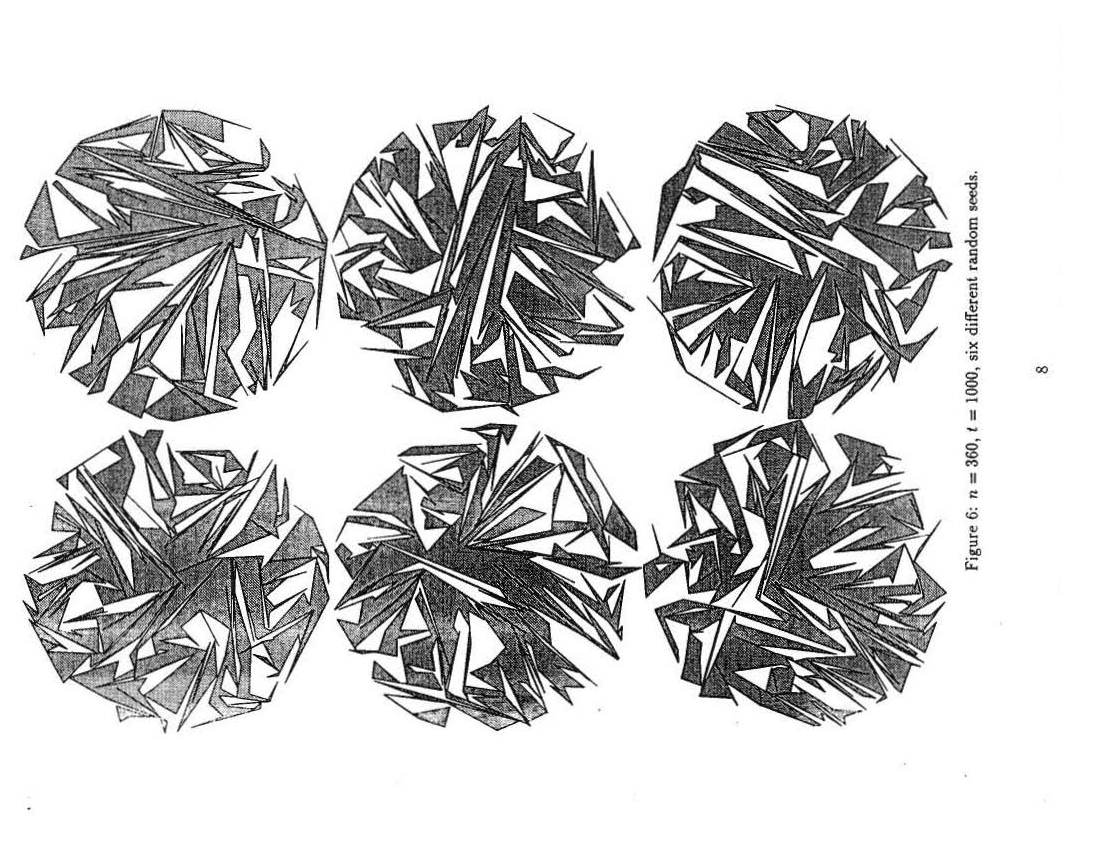
\includegraphics[width=0.90\textwidth]{velocity_sample.png}
  \end{center}
\end{frame}

\begin{frame}{Generation algorithms}
  Random Polygon Algorithm \begin{footnotesize}by Dailey and Whitfield\end{footnotesize}
  \vspace*{1em}
  \begin{itemize}\begin{small}
    \item[ ] input: size n
    \item[i.] generate 3 random points $ \rightarrow $ random n-gon P size 3
    \item[ii.] randomly choose and discard edge $ \overline{ab} $
    \item[iii.] determine region P' in polygon visible from $ \overline{ab} $
    \item[iv.] randomly choose point c in P'
    \item[v.] add edges $ \overline{ac} $, $ \overline{bc} $ to polygon P
  \end{small}\end{itemize}
  \vspace*{1em}
  \begin{itemize}\begin{small}
    \item main reason for geometry framework
    \item nontrivial problem to determine visible region P'
    \item most complex of all generation algorithms
  \end{small}\end{itemize}
\end{frame}

\begin{frame}{Nontrivial resulting algorithmic problems}
  \begin{itemize}\begin{small}
    \item order of points representing polygon: cc-wise
    \item triangularization
    \item random point in polygon
    \item intersection line with polygon
    \item surface area of polygon
  \end{small}\end{itemize}
\end{frame}

\begin{frame}{Demonstration GUI}
  \begin{itemize}\begin{small}
    \item basic version
    \item next important step:
      better way to pass parameters
  \end{small}\end{itemize}
\end{frame}

\begin{frame}{Again Milestones}
  This Milestone:
  \begin{itemize}\begin{small}
    \item 2 polygon generation algorithms missing
    \item shortest path generator missing
    \item possible in 1 week
  \end{small}\end{itemize}
  \vspace*{1em}
  Next Milestone:
    \begin{itemize}\begin{small}
      \item history objects
      \item step-by-step visualization
      \item statistic backend
    \end{small}\end{itemize}
\end{frame}

\end{document}

